\documentclass[preprint,12pt,authoryear]{elsarticle}
\usepackage{lmodern}
\usepackage[UTF8,fontset=none,heading=false,scheme=chinese]{ctex}
\setCJKmainfont[BoldFont=Noto Serif CJK SC Bold]{Noto Serif CJK SC}
\setCJKsansfont{Noto Sans CJK SC}
\setCJKmonofont{Noto Sans Mono CJK SC}
\abstracttitle{摘要}
\keywordtitle{关键词}
\renewcommand{\figurename}{图}
\renewcommand{\tablename}{表}
\renewcommand{\refname}{参考文献}
\usepackage{amsmath,amssymb}
\usepackage{graphicx}
\usepackage{booktabs,tabularx,array,adjustbox,longtable}
\usepackage[hidelinks]{hyperref}
\usepackage{xcolor}
\usepackage{float}
\usepackage{fvextra}
\usepackage{lineno}
\linenumbers
\providecommand{\tightlist}{\setlength{\itemsep}{0pt}\setlength{\parskip}{0pt}}
\newcommand{\pandocbounded}[1]{#1}
\setlength{\tabcolsep}{4pt}
\renewcommand{\arraystretch}{1.15}
\biboptions{sort,semicolon}
\journal{Computers and Electronics in Agriculture}
% first page: page number only in the footer, so the corresponding-author note has room
\makeatletter
\def\ps@pprintTitle{\let\@oddhead\@empty\let\@evenhead\@empty
  \def\@oddfoot{\reset@font\hfil\thepage\hfil}\let\@evenfoot\@oddfoot}
\makeatother

\makeatletter\patchcmd{\printFirstPageNotes}{Email address:}{电子邮箱：}{}{}\makeatother
\begin{document}
\begin{frontmatter}
\title{基于作业记录校准行间重叠量以控制农田全覆盖作业的漏作业概率}
\author[a]{［作者 1］\corref{cor1}}
\ead{［电子邮箱］}
\author[b]{［作者 2］}
\author[a]{［作者 3］}
\cortext[cor1]{通讯作者。}
\newpageafter{author}
\affiliation[a]{organization={[Department, Institution]}, city={[City]}, postcode={[Postcode]}, country={[Country]}}
\affiliation[b]{organization={[Department, Institution]}, city={[City]}, postcode={[Postcode]}, country={[Country]}}

\begin{abstract}
避免相邻行程间漏作业所需的重叠量取决于 GNSS 接收机、地形、农机具和控制器，而生产中的固定重叠量无法说明漏作业概率有多大。为此，本文提出共形收缩法，由田间作业记录校准重叠裕量。该方法为导航终端给出一个行距设定值，使一次作业留下任何漏作业带的概率低于选定水平；对于其他任一裕量，也能给出相应的漏作业概率。每次作业记录归结为一个覆盖分数，即该次作业实际行程不留任何漏缝的最小裕量；裕量取这些分数的某一次序统计量。有作业历史的田块用自身记录校准；无作业历史的田块则从众多其他田块各取一次作业记录，经车辆---地形---GNSS 模型归一化后校准。这一概率上界不需要对误差分布作假设，只要求各次作业或各田块可交换。以真实田块边界、地形和 GNSS 误差驱动的预注册仿真表明：除导航使前后相继的行程相互耦合，或实施裕量超过校准所用基准裕量的情形外，均达到目标漏作业水平。每块田有 100 次作业记录时，本方法的重叠率比两种共形规划方法低 4\%～55\%；无目标田块记录时，其重叠率比逐田块最优值高 0.6 个百分点，而其他基线方法高 1.2～4.4 个百分点。仅当单位面积漏作业损失约为重复作业损失的 40～90 倍时，零漏作业裕量才优于厂商经验规则。
\end{abstract}

\begin{keyword}
全覆盖路径规划；行间精度；重叠量；GNSS 导航；共形预测；精准农业
\end{keyword}
\end{frontmatter}

\section*{符号与缩写}
{\footnotesize
\begin{tabularx}{\textwidth}{@{}>{\raggedright\arraybackslash}p{0.24\textwidth}X@{}}
\toprule
\textbf{符号 / 缩写} & \textbf{含义} \\
\midrule
\(w\) & 农机具作业幅宽（作业带宽度） \\
\(W\) & 作业主区：田块边界向内收缩 \(2w\) 后的区域（其余为地头） \\
\(\lambda\) & 裕量：相邻行程的规划重叠量为 \(2\lambda\)，导航行距为 \(w-2\lambda\) \\
\(\pi(\lambda)\), \(K(\lambda)\) & 裕量为 \(\lambda\) 的等行距规划及其行程数 \\
\(J(\lambda)\) & \(\pi(\lambda)\) 在作业主区的重叠率 \\
\(e_k(x)\) & 第 \(k\) 个实际行程在沿行程位置 \(x\) 处的横向偏移 \\
\(M(\lambda,e)\) & 作业主区内的漏作业（未作业）面积 \\
\(c_i\); \(\ell\), \(u\) & 某一截面上按顺序排列的各实际行程中心；作业主区弦的两端 \\
\(r^\star(x)\) & 截面 \(x\) 处的覆盖半径（第 3.3 节） \\
\(S\) & 一次作业的覆盖分数（第 3.3 节） \\
\(\lambda_\mathrm{ref}\) & 记录覆盖分数所用基准规划的裕量 \\
\(\varepsilon\), \(\delta\) & 允许的一次作业出现漏作业带的概率；PAC 规则的置信参数 \\
\(n\), \(k_\star\) & 校准作业（或校准田块）数；用作裕量的次序统计量的秩 \\
\(q^\star\) & CE 验证批次覆盖分数的次序统计量 \(S_{(k_\star)}\) \\
\(\lambda^\star_f\) & 田块 \(f\) 的理想裕量：测试作业的无漏作业率 \(\ge1-\varepsilon\) 的最小裕量 \\
\(\hat q_f\) & 模型尺度：模型预测的田块 \(f\) 覆盖分数 \((1-\varepsilon)\) 分位数 \\
\(V_i\), \(v^\star\) & 归一化覆盖分数 \(S_i/\hat q_{f_i}\)；其次序统计量（第 3.5 节） \\
\(z\), \(\sigma(z)\), \(t\) & 探测线上 XTE 的 RMS；CE+ 的归一化函数；\(S/\sigma(z)\) 的共形分位数 \\
\(\kappa\) & 实施规划行程数少于基准规划时漏作业水平的放大系数（第 3.8 节） \\
\(\tau\), \(r\), \(r_\mathrm{be}\) & 漏缝容许宽度；成本比（单位面积漏作业损失与重复作业损失之比）；盈亏平衡成本比 \\
CE, CE-q, CE+ & 用田块自身作业记录校准的共形收缩法（Table~\ref{tab:2}） \\
XCE, XCE-T, XCE-MC & 跨田块共形收缩法；分别以解析（基于理论的）模型尺度和蒙特卡洛模型尺度归一化的跨田块共形收缩法 \\
CPrP, UBCP & 对比方法：共形预测规划 \citep{zhao2024}；基于联合界的共形规划，行程对层面 \citep{lindemann2023} \\
CQR & 共形分位数回归 \citep{romano2019} \\
BCD, CPP & 牛耕式单元分解；全覆盖路径规划 \\
LQR-I, MPC & 带积分环节的线性二次型调节器；模型预测控制 \\
RTK, DGPS, PPK & 实时动态、差分和后处理动态 GNSS 定位 \\
CORS & 连续运行参考站 \\
XTE, RMS & 自动导航系统输出的横向偏差；均方根 \\
PAC & 概率近似正确（对校准数据以 \(1-\delta\) 概率成立） \\
pp & 百分点 \\
\bottomrule
\end{tabularx}}

\section{引言}

施药、施肥、播种和耕整等田间作业通常按平行行程规划，行距等于农机具作业幅宽减去重叠量。实际作业中，GNSS 定位误差、坡地和湿软土壤上的车轮打滑、侧坡引起的天线横滚、安装偏差以及转向控制器的有限带宽，都会使实际行程偏离规划线。当相邻两行程的偏离之差超过二者的重叠量，或最外侧行程偏离田块边界时，就会留下漏作业带。因此，起决定作用的是相邻行程之间的相对误差，即行间精度（pass-to-pass accuracy）。漏作业和重叠都有代价：漏作业带导致减产或病虫草害得不到防治，重叠则使种子、化肥和农药被重复施用 \citep{fao2025,zhang2015,zhang2021}。无人驾驶农机作业时，没有驾驶员发现并修补漏缝，裕量必须事先设定正确。

现行做法是设定固定的重叠量，通常取厂商标称行间精度的两倍，或凭经验确定。这样设定的裕量既不能说明漏作业概率，也不能随田块形状、地形、接收机等级或作业幅宽调整。全覆盖路径规划（coverage path planning, CPP）研究假设农机严格按规划执行 \citep{galceran2013,hoffmann2024}；控制领域的研究减小了跟踪误差，但没有说明漏作业会以多大频率发生 \citep{lenain2006}。共形预测（conformal prediction）可直接由作业记录确定裕量，所给保证在有限样本下成立，且不需要对误差分布作假设；该方法已被用于路径规划 \citep{lindemann2023,zhao2024}，但尚未用于农田全覆盖作业。与已有应用相比，农田全覆盖作业有以下三个特点。

（1）只有每一对相邻行程和每一段田块边界都被覆盖，一次作业才无漏作业，因此保证必须同时对众多行程对中的最坏情形成立。

（2）记录数据所用的行距与最终实施的行距不同。行距越窄，行程越多，出现漏缝的机会也越多，因此在某一行距下测得的可靠性不能直接推广到更窄的行距。

（3）一块田每年只作业寥寥数次，而在 10\% 的漏作业水平下，共形裕量至少需要同一田块的 9 次作业记录；若要求保证对实际记录到的这批作业以 0.9 的置信度成立，则至少需要 22 次。

针对上述问题，\textbf{本文提出共形收缩法（conformal erosion）}，由作业记录校准全覆盖规划的重叠量。``收缩''是指在规划每一行程时，假定农机具两侧各窄了裕量 \(\lambda\)，从而在相邻行程之间留出 \(2\lambda\) 的重叠量。方法的输出是可直接输入导航终端的行距设定值 \(w-2\lambda\)，同时给出按该设定作业时留下任何漏作业带的概率；反之，对于用户偏好的任一裕量，同一批数据也能给出其漏作业概率。方法流程见图~\ref{fig:1}。本文的贡献分别对应上述三个特点：

\textbf{（1）精确的覆盖分数（第 3.3 节）。} 覆盖分数可判定一次作业是否留下漏作业带，田块边界也计算在内。由于它是所有此类分数中最小的，所得裕量不大于以往共形规划方法基于逐行程对分数所得的裕量（对应特点（1））。

\textbf{（2）有作业历史田块的校准（第 3.4 节和第 3.6 节）。} 校准所用作业记录取自基准规划，其行程数不少于实施规划；推广检查确保这一大小关系成立（对应特点（2））。

\textbf{（3）无作业历史田块的校准（第 3.5 节）。} 农场或农机作业服务组织通常管理大量田块，每块田只有一两次作业记录。本方法从每块田各取一次作业记录合并校准；车辆---地形---GNSS 模型的计算不使用作业数据，只用于把各田块归一到统一尺度（对应特点（3））。

\textbf{（4）预注册仿真评估（第 3.9 节和第 4 节）。} 每项实验使用 30～135 块未参与校准的田，对比对象包括共形规划方法、生产经验规则、考虑机型配置的基线方法和机器学习预测方法，并开展了稳健性检验和成本分析。

\begin{figure}[!htbp]
\centering
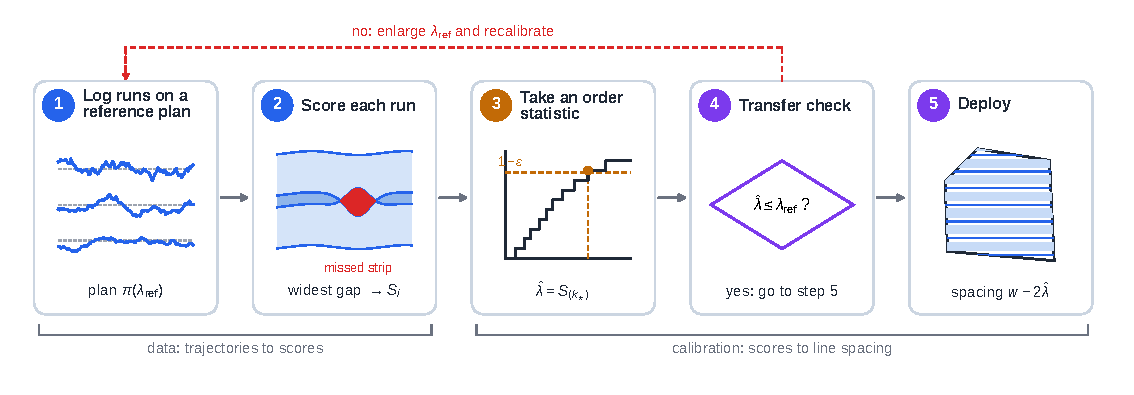
\includegraphics[width=\textwidth]{../../../figures/paper/fig_workflow.pdf}
\caption{本文方法流程。作业记录来自目标田块，或来自众多其他田块（每块田一次），每次作业记录归结为一个覆盖分数（步骤 2）；取这些分数的某一次序统计量作为裕量，若分数来自其他田块，则先除以不使用作业数据计算的模型尺度（步骤 3）；再由用户的规划器生成实施规划（步骤 4）。推广检查：若 \(\hat\lambda>\lambda_\mathrm{ref}\)，则在裕量更大的基准规划上重新校准。}\label{fig:1}
\end{figure}

所有验证性实验均已预注册：实验方案和判定准则在实验运行前存入带时间戳的代码仓库，以免事后挑选结果。未达成和部分达成的预期结论与已达成的结论一并报告，事后分析均已标注（表 S20）。

\section{相关研究}

\textbf{全覆盖路径规划。} 结合作业方向优化的牛耕式单元分解（boustrophedon cellular decomposition, BCD）是农田全覆盖规划的标准方法 \citep{hoffmann2024}。Fields2Cover 提供了包含航向搜索和 Dubins 转弯的开源实现 \citep{mier2023}，\citet{mier2025} 进一步加入了连续曲率的地头路径，\citet{hameed2016} 则计算了与 3D 地形等效的行距。这些方法都没有给出完全覆盖的概率；本文方法正是为这类规划器提供其所需的输入裕量。

\textbf{鲁棒裕量与基于模型的裕量。} 管道模型预测控制（tube MPC）\citep{mayne2005}、带 Rice 极值修正的高斯机会约束 \citep{rice1944}、高斯过程谨慎控制 \citep{hewing2020}、Wasserstein 分布鲁棒 CVaR \citep{mohajerin2018} 和场景法 \citep{campi2008} 借助模型、最坏情况或采样约束来界定跟踪误差。然而，RTK 误差呈重尾分布且大误差在时间上成簇出现，参数模型难以准确刻画其尾部（第 3.9 节）；最坏情况集合则过于保守。无偏差模型预测控制（offset-free MPC）\citep{pannocchia2003} 和打滑观测器 \citep{lenain2006} 能减小误差，但不能给出漏作业概率的上界。

\textbf{共形预测。} 本文方法建立在以下研究的基础上：分割共形预测及其训练条件（PAC）变体 \citep{vovk2012}；协变量偏移下以及超出可交换性条件的共形预测 \citep{tibshirani2019,barber2023}；共形分位数回归 \citep[CQR;][]{romano2019}；共形风险控制 \citep{angelopoulos2024crc,angelopoulos2025ltt}；每组仅有一个样本的分层共形预测 \citep{dunn2023}；以及函数型共形预测带 \citep{lei2015,diquigiovanni2022}，本文的覆盖分数即属于函数型共形预测带的一种。已有的共形规划方法 \citep{lindemann2023,zhao2024,sun2023,wang2025} 均未处理随规划变化的行程对最大值问题。

\section{材料与方法}

\subsection{问题描述}

\textbf{田块、规划与裕量。} 田块为一多边形。将田块向内收缩 \(2w\)（\(w\) 为作业幅宽）得到\textbf{作业主区} \(W\)，其余部分为地头；这只是评价时采用的约定，不影响方法本身。规划是沿作业方向 \(x\) 布置的一组直线行程中心线 \(y_1<\dots<y_K\)。给定\textbf{裕量} \(\lambda\ge0\)，规划器 \(\pi(\lambda)\) 从一侧边界起按行距 \(w-2\lambda\) 布置平行线，使相邻规划作业带重叠 \(2\lambda\)；行程数 \(K(\lambda)\) 随 \(\lambda\) 增大而不减。重叠率 \(J(\lambda)\) 定义为 \(W\) 内的作业带面积与 \(W\) 面积之比减 1。

\textbf{作业执行。} 第 \(k\) 个行程以横向偏移 \(e_k(x)\) 行驶，其在位置 \(x\) 处的作业带为 \([y_k+e_k(x)-w/2,\ y_k+e_k(x)+w/2]\)（图~\ref{fig:2}）。横向偏移是随机的，沿行程方向和行程之间均存在相关性：相邻行程读取的是同一条 GNSS 误差轨迹，只是相隔一个行程的时长。各行程行驶时所处的地形和时刻由规划决定，因此偏移还依赖于规划本身。覆盖情况在 \(W\) 的截面上评估，截面沿作业方向间隔 1 m。

\textbf{优化目标。} 记 \(M(\lambda,e)\) 为以偏移 \(e\) 执行 \(\pi(\lambda)\) 时 \(W\) 内的漏作业面积。理想情况下，应在一次作业不出现任何漏作业带的概率不低于 \(1-\varepsilon\) 的前提下，取最小的重叠率：
\[
\min_{\lambda}\ J(\lambda)\quad\text{s.t.}\quad \Pr\big[M(\lambda,e)=0\big]\ \ge\ 1-\varepsilon ,
\]
所有实验均取 \(\varepsilon=0.1\)。由于 \(e\) 的分布未知，上式的最优解，即田块 \(f\) 的\textbf{理想裕量} \(\lambda^\star_f\)，无法计算；本方法转而给出作业记录所能支持的最小裕量。

\begin{figure}[!htbp]
\centering
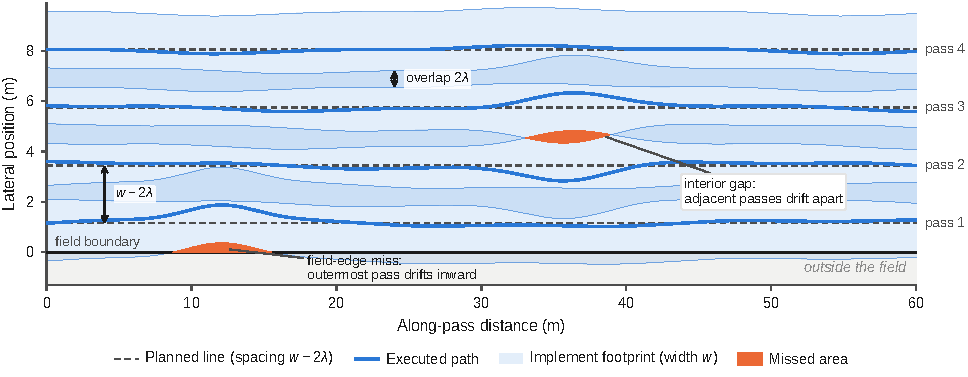
\includegraphics[width=\textwidth]{../../../figures/paper/fig_schematic.pdf}
\caption{覆盖问题示意。（a）DGPS 机型配置（R3，6 m 农机具；第 3.9 节）在一块真实水田上的一次仿真作业，按该田块的理想裕量规划；虚线内为作业主区，漏作业带（红色，宽度经放大）出现在相邻两行程偏离之差超过规划重叠量的位置。（b）方框区域局部放大，最大漏缝宽度为 12 cm。（c）某一沿行程位置处的横截面（示意）：只有当两个实际中心相距超过 \(w\)（内部漏缝），或最外侧中心距边界超过 \(w/2\)（边界漏作业）时，弦 \([\ell,u]\) 才未被完全覆盖。}\label{fig:2}
\end{figure}

\subsection{方法概述}

共形收缩法分 4 步由作业记录得到裕量（图~\ref{fig:1}）：

\begin{enumerate}
\def\labelenumi{\arabic{enumi}.}
\tightlist
\item
  \textbf{生成基准规划。} 用用户现有的规划器生成裕量较宽裕的基准规划 \(\pi(\lambda_\mathrm{ref})\)。作业记录取自该规划，或取自其他田块的基准规划。
\item
  \textbf{计算每次作业的覆盖分数。} 将农机具的实际轨迹归结为一个覆盖分数 \(S\)（第 3.3 节）。
\item
  \textbf{校准裕量。} 裕量 \(\hat\lambda\) 取覆盖分数的某一次序统计量，使新一次作业的分数超过它的概率不大于 \(\varepsilon\)；该结论或在对校准数据取平均的意义下成立（边际规则），或以 \(1-\delta\) 的置信度成立（PAC 规则）。覆盖分数取自田块本身（第 3.4 节）；对没有作业历史的田块，则从其他多个田块各取 1 次作业，并将其分数除以模型预测的尺度（第 3.5 节）。
\item
  \textbf{规划与实施。} 经推广检查确认 \(\hat\lambda\le\lambda_\mathrm{ref}\) 后，生成并实施 \(\pi(\hat\lambda)\)（第 3.6 节）。用户在导航终端中将行距设为 \(w-2\hat\lambda\)。
\end{enumerate}

表~\ref{tab:1} 和表~\ref{tab:2} 分别列出了用户需提供的输入和本方法的各变体。各变体的步骤 2 相同，区别在于：\(\lambda_\mathrm{ref}\) 如何选取，校准分数取自何处、如何归一化，以及实施规划是基准规划本身（CE）还是裕量更小的规划（CE-q、CE+、XCE）。

\begin{table}[!htbp]
\centering
\footnotesize
\caption{用户需提供的输入}\label{tab:1}
\begin{adjustbox}{max width=\textwidth}
\begin{tabular}{@{}l>{\raggedright\arraybackslash}p{20.8em}@{}}
\toprule
\textbf{输入} & \textbf{要求} \\
\midrule
规划器 & 可接受裕量，即按行距 \(w-2\lambda\) 布置行程 \\
作业记录 & 完整作业，记录农机具作业中心（而非拖拉机）的轨迹，轨迹来自精度远高于裕量的独立参考基准，例如安装在农机具上的 PPK 流动站；仅有导航日志不够 \\
数据合并条件 & 拖拉机、农机具、接收机、差分改正源、控制器参数和作业速度均相同，季节与土壤状态的构成相同；生产中会停机的作业段（如 RTK 失锁）在校准和使用时按同一方式处理 \\
作业次数 \(n\) & 每块田不少于 9 次（边际规则）或 22 次（PAC 规则）；XCE 为校准田块数 \\
基准裕量 & CE：由预试批次逐步提高；CE+、XCE：5 块训练田中覆盖分数 \((1-\varepsilon)\) 分位数最大值的 1.25 倍（R1～R3 分别为 17.5、19.4、43.4 cm） \\
\(\varepsilon\)、\(\delta\)、\(\tau\) & 在查看校准分数之前选定 \\
仅 XCE 需要 & 每块田的控制器参数、地形模型、GNSS 精度等级和作业幅宽；车辆仿真模型（数字孪生）或解析模型 \\
仅 CE+ 需要 & 5 块训练田；每次作业在 1 条地头探测线上记录的自动导航横向偏差（XTE） \\
输出 & \(\hat\lambda\)（行距 \(w-2\hat\lambda\)）或拒绝给出裕量；任一事先确定的裕量所对应的漏作业概率 \\
\bottomrule
\end{tabular}
\end{adjustbox}
\end{table}

\begin{table}[!htbp]
\centering
\footnotesize
\caption{本文方法的变体。CE-q 为核心变体，CE+ 为可选的改进。除 CE 外，各变体的实施裕量均须不大于 \(\lambda_\mathrm{ref}\)。}\label{tab:2}
\begin{tabularx}{\textwidth}{@{}l>{\raggedright\arraybackslash\hsize=0.95\hsize}X>{\raggedright\arraybackslash\hsize=1.03\hsize}Xl>{\raggedright\arraybackslash\hsize=1.03\hsize}X@{}}
\toprule
\textbf{方法变体} & \textbf{校准数据} & \textbf{分数尺度} & \textbf{实施规划} & \textbf{实施规划的保证} \\
\midrule
CE & 目标田块的作业（预试批次 + 验证批次） & 无 & 基准规划本身 & 不需要对误差分布作假设，只要求各次作业可交换（附录 A.4） \\
CE-q & 目标田块的 \(n\) 次作业 & 无 & \(\pi(\hat\lambda)\) & 同 CE，但在耦合假设下按 \(\kappa\) 放大（附录 A.15） \\
CE+ & 目标田块的 \(n\) 次作业 + 5 块训练田 & 探测线 XTE，通过交叉验证时采用 & \(\pi(t\,\sigma(z))\) & 对 \(S/\sigma(z)\) 成立；实施规划：在耦合假设下给出 \(P(S_\mathrm{new}>t\sigma(z_\mathrm{new})-\bar\Delta)\) 的上界（附录 A.9） \\
XCE-T / XCE-MC & 其他 \(n\) 块田各 1 次作业 & 模型分位数 \(\hat q_f\)（解析模型 / 蒙特卡洛数字孪生） & \(\pi(\hat q_g v^\star)\)，\(g\) 为目标田块 & 覆盖分数：不需要对误差分布作假设，只要求各田块可交换（附录 A.17）；实施规划：推广系数 \(\kappa\) \\
\bottomrule
\end{tabularx}
\end{table}

\subsection{单次作业的覆盖分数（步骤 2）}

直观地说，在每个截面上检查两件事：相邻两个实际行程是否相距超过一个作业幅宽，最外侧行程距边界是否超过半个作业幅宽；田块中最不利的位置决定该次作业所需的裕量。严格地，在截面 \(x\) 处，截面与 \(W\) 相交得到弦 \([\ell(x),u(x)]\)；记 \(c_1<c_2<\dots\) 为作业带与该弦相交的各行程的实际中心，再加上两侧各自最近的一个行程，\(Y(x)\) 为这些中心的集合。该弦被完全覆盖，当且仅当
\[
r^\star(x)=\max\Big\{\mathrm{dist}(\ell,Y),\ \mathrm{dist}(u,Y),\ \max_{i:\ (c_i+c_{i+1})/2\in[\ell,u]}\tfrac12(c_{i+1}-c_i)\Big\}\ \le\ \tfrac w2 ,
\]
式中前两项为边界项，第三项为相邻行程间最大漏缝宽度的一半。对基准规划的一次作业，\textbf{覆盖分数}定义为
\[
S=\lambda_\mathrm{ref}+\max_x\big(r^\star(x)-w/2\big).
\]
覆盖分数针对实际执行的规划，度量在出现漏作业带之前，所有实际作业带还能收窄多少（\(S<\lambda_\mathrm{ref}\)）或必须加宽多少（\(S>\lambda_\mathrm{ref}\)）：一次作业无漏作业，当且仅当 \(S\le\lambda_\mathrm{ref}\)。若要把 \(S\) 理解为另一规划所需的裕量，则需要耦合假设（第 3.8 节）。

无论误差过程如何，覆盖分数都能精确判定作业主区是否被完全覆盖（附录 A.1）。在所有能在任一裕量下（即对实际作业带作任意虚拟加宽或收窄时）判定完全覆盖的分数中，覆盖分数是最小的（附录 A.3）。因此，对相同的作业记录和校准规则，由它得到的裕量不大于任何其他此类分数得到的裕量，以往共形规划方法所用的逐行程对最大值也包括在内。内部漏缝取决于两个行程之差，相邻行程的共同误差在其中相互抵消；边界项则承受单个行程的全部误差，因此其离散程度至少为前者的 \(\sqrt2\) 倍。由边界项决定覆盖分数的频率见第 4.3 节。

\subsection{利用本田块作业记录校准（步骤 3a；CE、CE-q、CE+）}

将 \(n\) 个覆盖分数从小到大排序。\textbf{边际规则}取其中第 \(k_\star\) 个，\(k_\star=\lceil(n+1)(1-\varepsilon)\rceil\)，例如 30 个分数取第 28 个；此时在对作业记录取平均的意义下，新一次作业超过该值的比例不大于 1/10。\textbf{PAC 规则}取满足 \(\mathrm{BinomCDF}(k_\star-1;n,1-\varepsilon)\ge1-\delta\) 的最小 \(k_\star\)：对实际记录的这批作业，漏作业概率不大于 \(\varepsilon\) 这一结论以 \(1-\delta\)（本文取 0.9）的置信度成立。若 \(k_\star>n\)，则不实施任何规划；当 \(\varepsilon=\delta=0.1\) 时，两种规则分别要求 \(n\ge9\) 和 \(n\ge22\)。

\textbf{CE。} CE 先搜索足够大的基准裕量，再加以验证：（1）在 \(\pi(\lambda_\mathrm{ref})\) 上记录一批预试作业，计算其覆盖分数的 \((1-\varepsilon)\) 经验分位数 \(q\)；（2）若 \(q>\lambda_\mathrm{ref}\)，令 \(\lambda_\mathrm{ref}=1.10\,q\)，重复第（1）步；（3）固定该规划，再记录一批验证作业；（4）若验证作业的次序统计量 \(q^\star=S_{(k_\star)}\) 不大于 \(\lambda_\mathrm{ref}\)，则实施 \(\pi(\lambda_\mathrm{ref})\)，否则不实施任何规划。实施规划就是计算覆盖分数所用的规划，因此 CE 除作业可交换外不需要其他假设。

\textbf{CE-q。} CE-q 实施 \(\pi(q^\star)\)，其行程数不多于基准规划，重叠率也不高于基准规划。

\textbf{CE+。} CE+ 将作业预算固定为 \(n\) 次，基准裕量 \(\lambda_\mathrm{ref}\) 取自训练田块（表~\ref{tab:1}），并可用预测尺度 \(\sigma(z)\) 对每个覆盖分数归一化。该尺度是一个线性函数，其自变量为均方根 \(z\)：田内行程开始前，农机先沿地头行驶一条探测线，记录自动导航横向偏差（XTE）并求其均方根。CE+ 实施的裕量为 \(t\,\sigma(z_\mathrm{new})\)，其中 \(t\) 为 \(S_i/\sigma(z_i)\) 的共形分位数。XTE 反映的是打滑和地面粗糙度，而不是 GNSS 误差，因为接收机感知不到自身的 GNSS 误差。只有当这一归一化在训练田块的留一田块交叉验证中使平均裕量降低至少 3\% 时才采用（各常数见附录 C.5）。

\textbf{算例。} R1 中的 440 号田块（\(w=3\) m）基准裕量为 17.5 cm，有 \(n=29\) 次作业记录，因此 \(k_\star=27\)。覆盖分数为 4.5～16.5 cm（中位数 7.0 cm），第 27 小的为 9.4 cm。因此，CE-q 实施的裕量为 9.4 cm，即行距 281.1 cm，作业主区重叠率 6.97\%。该田块的理想裕量为 10.7 cm（重叠率 7.58\%）。就这一组 29 次作业而言，测试作业的无漏作业率为 0.745；对 29 次作业重复抽样 2000 次，无漏作业率的平均值为 0.890（第 10～90 百分位数为 0.811～0.963）。每个测试估计值本身仅基于 200 次作业，考虑到这一点，该结果与目标值 0.9 接近。上述界在对作业记录取平均的意义下成立，并非对每一组作业记录都成立；用户若需要该界对自己的特定作业记录也成立，应采用 PAC 规则。

\subsection{跨田块校准（步骤 3b；XCE）}

对于没有作业记录的目标田块 \(g\)，XCE 从其他 \(n\) 个田块各取 1 次作业合并校准。\textbf{模型尺度} \(\hat q_f\) 根据控制器参数、地形模型和 GNSS 精度等级，预测各田块基准规划上覆盖分数的 \((1-\varepsilon)\) 分位数，\textbf{不使用任何作业数据}。XCE 对每个校准田块计算 \(V_i=S_i/\hat q_{f_i}\)，取其边际或 PAC 次序统计量 \(v^\star\)，目标田块的裕量为 \(\lambda_g=\hat q_g\,v^\star\)。若某田块的预测失败（\(\hat q_{f_i}\) 不是有限值），则令 \(V_i=+\infty\)，此时目标田块不实施任何规划。

任何仅由田块属性计算的尺度，都能保持覆盖分数层面的田块平均保证；模型的精度决定裕量的松紧，以及无漏作业率在各田块和各机型配置之间分布的均匀程度。用于对比的尺度包括：直接合并（\(\hat q\equiv1\)）、按机型配置分组合并（Mondrian 共形）、厂商规格尺度、学习得到的 CQR 型岭回归尺度 \citep{romano2019} 以及按机型配置的经验尺度。最后一种由校准田块自身的覆盖分数估计，其有效性只能通过实验检验。

\emph{XCE-MC} 在基准规划上运行 1000 次闭环车辆仿真（即数字孪生），取覆盖分数的 0.9 分位数。\emph{XCE-T} 用解析方法计算同一个量（附录 B）：将闭环系统沿无噪声路径线性化，给定作业条件时，每个行程的横向误差服从高斯分布；漏缝超过阈值的概率用 Kac--Rice 上穿和求上界，或用高斯蒙特卡洛抽样估计；田块边界的超限概率以各单行程概率之积为上界，此时将每个行程起点的状态视为已知（附录 A.10、附录 A.12）；最后合成各行程对，并对 200 种作业条件求混合。XCE-T 以 Kac--Rice 公式 \citep{azais2009,piterbarg1996}、平稳过程极值理论 \citep{leadbetter1983,hall1979} 和统计线性化 \citep{booton1954,kazakov1956} 为基础。两种实现均对每块田离线计算一次：XCE-T 在单核上不计边界项时每块田耗时 16～353 s（表 S21），计入边界项时耗时中位数为 271 s（129～2356 s；附录 B.3）；XCE-MC 的耗时中位数为 8～21 s（共享的四核计算机）。

\subsection{实施与推广检查（步骤 4）}

对于实施规划不是基准规划的各变体（CE-q、CE+ 和 XCE），实施裕量不得大于 \(\lambda_\mathrm{ref}\)；否则实施规划的行程数将多于记录覆盖分数所用的规划，可靠性保证不再适用。若 \(\hat\lambda>\lambda_\mathrm{ref}\)，则 \(\pi(\hat\lambda)\) 和基准规划都不实施（校准结果已表明 \(\lambda_\mathrm{ref}\) 过小），而是在裕量更大的基准规划上对该田块重新校准：CE 提高 \(\lambda_\mathrm{ref}\) 后记录新的预试批次；XCE 以更大的裕量重新生成各基准规划，并重新计算模型尺度。预注册实验未包含这一检查；第 4.1 节和第 4.3 节给出了该检查本应触发的频率。

\subsection{\texorpdfstring{漏缝容许宽度与 \(\varepsilon\) 的选取}{漏缝容许宽度与 \textbackslash varepsilon 的选取}}

有些作业允许存在较窄的未作业带，例如喷杆末端喷嘴的喷量逐渐递减，可由相邻行程弥补。此时，需要控制的事件可放宽为``不存在宽于 \(\tau\) 的漏缝''。内部漏缝宽度为 \(2(r^\star-w/2)\)，边界漏作业带宽度为 \(r^\star-w/2\)，因此 \(S_\tau=S-\tau/2\) 仍是有效的覆盖分数（对边界漏作业带偏保守），相应裕量为 \(\hat\lambda-\tau/2\)。矩形作业带适用于整个作业幅宽内作业均匀的情形（如喷杆喷雾、旋耕）；播种和离心式撒肥则需另行定义覆盖分数。水平 \(\varepsilon\) 属于经济决策（第 4.4 节）。\(\varepsilon\) 和 \(\tau\) 必须在查看覆盖分数之前确定；若根据同一批覆盖分数按成本选取，边际保证即不再成立，除非改用对所有裕量同时成立的界（如 DKW 置信带）。

\subsection{可靠性保证的前提}

对用户而言：（1）直接实施记录作业所用的规划最为稳妥；（2）实施规划的行距可以更宽（行程更少），但不能更窄；（3）跨田块保证是对整个机队的平均，因此须逐一检查各机型配置。严格表述见附录 A。

\begin{itemize}
\tightlist
\item
  \textbf{覆盖分数。} 在已知农机具位置真值的条件下，对作业主区按 1 m 间距划分的截面网格，覆盖分数对区间型作业带是精确的（附录 A，F1～F2）。
\item
  \textbf{作业可交换（CE）。} 作业记录与新一次作业可交换（PAC 规则要求独立同分布），即季节、土壤状态和 GNSS 条件的构成相同，且不存在趋势变化或设备更换。边际规则保证 P(实施且漏作业) \(\le\varepsilon\)，该概率是对校准数据取平均的结果；PAC 规则则以对校准数据 \(1-\delta\) 的概率保证：在实施的条件下，漏作业概率不大于 \(\varepsilon\)（附录 A.4）。
\item
  \textbf{行程更多的规划。} 行程更多的规划，其覆盖分数通常在随机序意义下更大。因此，若像以往共形规划方法那样在标称规划 \(\pi(0)\) 上校准阈值，该阈值对实施规划没有不依赖分布的保证。以行程对分数独立同分布为例，标称规划有 \(K_0\) 个行程对、实施规划有 \(K_1>K_0\) 个行程对时，该阈值下的无漏作业率约为 \((1-\varepsilon)^{K_1/K_0}<1-\varepsilon\)（附录 A.6）。
\item
  \textbf{耦合假设（CE-q、CE+、XCE）。} 若实施规划的每个漏缝项或边界项，比基准规划中与之耦合的对应项超出的量不大于一个与噪声无关的量，则保证可推广到行程更少的规划。此时，对 CE-q 和 XCE，漏作业水平的放大倍数不大于 \(\kappa\)；本文未估计 \(\kappa\)，当规划改变引起的地形和时序效应较小时，该系数也较小（附录 A.15）。对线性闭环系统，若随规划变化的只有确定性响应，该假设成立；若重新排时使各行程读取的 GNSS 误差发生偏移，该假设近似成立；若导航系统使每个行程相对前一行程转向，该假设不成立。对采用非常数归一化尺度的 CE+，相应的界为 \(P(S_\mathrm{new}>t\sigma(z_\mathrm{new})-\bar\Delta)\)（附录 A.9）。
\item
  \textbf{田块可交换（XCE）。} 若各田块可交换（PAC 规则要求独立同分布），每个校准田块在其基准规划上提供 1 次作业，且归一化尺度只取决于田块属性，则无论模型精度如何，覆盖分数层面的保证都成立（附录 A.17），这与 \citet{dunn2023} 的两层设定相同。该保证是对校准田块、其作业和目标田块三者取平均：若作业记录集合固定、田块独立同分布，则目标田块上的平均无漏作业率是 \(\mathrm{Beta}(k_\star,n+1-k_\star)\) 的一次抽样（\(n=29\) 时标准差为 0.054）。它不是针对单个田块或单一机型配置的结论。
\item
  \textbf{理想尺度。} 即使以各田块的理想裕量作为尺度，目标田块的裕量仍等于其自身所需裕量乘以田块内尾部比值的一个次序统计量，该次序统计量由 \(n\)、\(k_\star\) 和田块内覆盖分数的分布决定。这是理想尺度下的恒等式，而不是对所有尺度都成立的下界：在一组实验条件下，不经归一化直接合并校准的代价反而低于理想尺度（附录 A.20）。
\end{itemize}

\subsection{仿真实验设计}

\textbf{数据来源。} 全部输入数据均为公开数据。田块边界和作业方向取自中国国家农机作业平台的 250 条联合收割机 GNSS 轨迹 \citep{wu2023}。采用基于密度的聚类从中提取田块 964 个，经筛选后选用水田 137 块（南方丘陵区）和麦田 162 块（华北平原）。地形数据取自 Copernicus GLO-30 \citep{esa2021}。GNSS 误差取自 12 对 NOAA CORS 站点（基线长 5～30 km，位于美国中西部和大平原），每对站点在 2024～2025 年四个季节中共取 8 d 数据。数据用 RTKLIB \citep{takasu2009} 的 demo5 分支 \citep{everett_demo5} 按移动站模式解算，得到 4 种接收机精度等级的误差序列（表~\ref{tab:3}）。30 s 历元的误差序列插值至 1 Hz 后，再叠加一条车载 GNSS/INS 记录 \citep{tang2022} 的高频残差。

\begin{table}[!htbp]
\centering
\footnotesize
\caption{CORS 解算序列的水平误差（每个精度等级 96 个站对---日）。RTK 误差的尾部来自持续数分钟的错误固定解和浮点解漂移，导航终端会对这类情况给出警示；若按 RMS 相同的高斯分布估计，误差超过 99.9\% 分位数的概率会被低估若干个数量级。静态天线不受车载多路径效应影响，也不存在差分链路中断。}\label{tab:3}
\begin{adjustbox}{max width=\textwidth}
\begin{tabular}{@{}l>{\raggedright\arraybackslash}p{20.8em}llll@{}}
\toprule
\textbf{精度等级} & \textbf{解算方式} & \textbf{RMS} & \textbf{95\%} & \textbf{99.9\%} & \textbf{最大值} \\
\midrule
RTK & 载波相位，模糊度解算（固定解历元占 84\%，浮点解占 16\%） & 2.4 cm & 3.3 cm & 24.5 cm & 1.39 m \\
RTK 浮点解 & 载波相位，不解算模糊度 & 2.6 cm & 4.0 cm & 24.6 cm & 1.39 m \\
DGPS & 伪距差分 & 32.5 cm & 57.8 cm & 2.05 m & 6.05 m \\
单点定位 & L1 伪距 & 1.51 m & 2.78 m & 4.97 m & 7.16 m \\
\bottomrule
\end{tabular}
\end{adjustbox}
\end{table}

\textbf{仿真模型。} 闭环仿真模型的时间步长为 0.05 s，车速为 2 m/s，包含以下环节：（1）运动学转向模型，转向滞后 0.25 s，转角饱和值 35°，转向速率限制 30°/s；（2）地形侧滑，与横向坡度成正比，并叠加 Ornstein--Uhlenbeck 过程描述的地面粗糙度，二者均按每次作业的土壤含水率缩放；（3）天线高 2.6 m，横滚（地形）补偿系数 \(0.85\pm0.05\)；（4）每次作业的安装偏差（标准差 1.5 cm）；（5）横向 GNSS 误差。各行程按时间顺序执行，含地头转弯。默认控制器为带积分环节的 LQR（LQR-I）；作业带以车辆参考点为中心，对应刚性悬挂农机具。详见附录 C。

\begin{table}[!htbp]
\centering
\footnotesize
\caption{机型配置。混合机队合并全部 3 种配置。水田坡度取自 30 m 分辨率高程模型，无法分辨经平整的田格。}\label{tab:4}
\begin{adjustbox}{max width=\textwidth}
\begin{tabular}{@{}lllll>{\raggedright\arraybackslash}p{7.3em}@{}}
\toprule
\textbf{机型配置} & \textbf{田块} & \textbf{GNSS 精度等级} & \textbf{幅宽 \(w\)} & \textbf{土壤含水率} & \textbf{厂商标称行间精度} \\
\midrule
R1 RTK，平地，3 m & 麦田（平原） & RTK & 3 m & Beta(2, 3) & 2.5 cm \\
R2 RTK，丘陵湿地，1.5 m & 水田（丘陵） & RTK & 1.5 m & 0.6～0.9 & 2.5 cm \\
R3 DGPS，丘陵，6 m & 水田（丘陵） & DGPS & 6 m & Beta(2, 3) & 20 cm \\
\bottomrule
\end{tabular}
\end{adjustbox}
\end{table}

\textbf{评价指标。} \emph{无漏作业率}指漏作业面积为零的测试作业所占比例，各田块合并计算；文中``覆盖''一词仅指面积覆盖。\emph{达标率}指 200 次测试作业中无漏作业率不显著低于 0.9 的田块所占比例（单侧二项检验，显著性水平 0.05）；由于各田块的校准结果随其校准作业而波动，校准正确的边际方法也只能在约 85\% 的田块上达标，PAC 方法约为 99\%（附录 A.19）。\emph{重叠率}指作业主区的重叠率 \(J\)；\emph{漏作业面积}指作业主区中未作业部分所占比例的均值；\emph{超额重叠率}指重叠率与该田块理想裕量规划重叠率之差，以百分点（pp）计。理想裕量是测试作业上无漏作业率达到 0.9 的最小裕量；它用到了测试分布，只作参照，并非一种方法。

\textbf{实验方案。} 田块按序号划分，使每项验证性实验所用田块均未用于设计该实验的分析（附录 C.2）。表~\ref{tab:5} 列出各研究问题及对应的实验；表 S20 列出每项实验对应的预注册文件。

\begin{table}[!htbp]
\centering
\footnotesize
\caption{仿真研究的问题及对应实验}\label{tab:5}
\begin{tabularx}{\textwidth}{@{}>{\raggedright\arraybackslash\hsize=1.00\hsize}X>{\raggedright\arraybackslash\hsize=1.00\hsize}Xll@{}}
\toprule
\textbf{研究问题} & \textbf{实验} & \textbf{性质} & \textbf{章节} \\
\midrule
有田块作业历史时，保证是否成立，裕量是否比共形规划方法更紧？ & A1：每种机型配置 30 块新田，每块田 100 次作业 & 预注册 & 4.1 \\
作业记录很少时代价多大？ & A2：\(n=9\)～100，每种机型配置 45 块田 & 预注册 & 4.1 \\
模型尺度的精度如何？ & 模型与 200 次作业分位数对比；B6 学习型预测器 & 描述性；事后分析 & 4.2 \\
无田块作业历史时，保证在总体和各机型配置下是否成立，是否高效？ & B1～B3 早期设计；B4 重复抽样；B5 混合机队 & 预注册 & 4.2 \\
方法对模型误差的敏感性如何？ & C1：6 种仿真真实场景变体 & 预注册 & 4.3 \\
地头绕行是否改变田块边界的作用？ & C2 & 预注册 & 4.3 \\
零漏作业裕量何时值得付出相应的重叠代价？ & 成本分析 & 描述性 & 4.4 \\
\bottomrule
\end{tabularx}
\end{table}

\section{结果}

\subsection{有作业历史的田块}

覆盖分数的判定与漏作业面积的结果逐次一致：在 6 块田上各仿真 200 次作业，每次作业的覆盖分数都复现了漏作业面积给出的结果（附录 A.3）。

\textbf{A1：预注册对比。} 两项预注册结论在所有机型配置中均成立（表~\ref{tab:6}）：一是 CE+ 有效；二是在两种规则下，CE+ 的作业主区重叠率均低于共形预测规划（CPrP）和行程对层面的联合界共形规划（UBCP）。所有方法每块田均使用 100 次作业记录，单块田很少能积累这么多记录；规划与控制均采用 BCD + LQR-I 组合。各机型配置的超额重叠率见图 S4。

\begin{table}[!htbp]
\centering
\footnotesize
\caption{实验 A1 结果（预注册；每种机型配置 30 块新田）。预注册结论：CE+ 边际规则的无漏作业率不显著低于 0.9（按田块聚类的 p 为 0.70、0.98、0.29）；CE+ PAC 在 30 块田中未通过达标检验的少于 9 块（各配置均为 0 块）；CE+ 的重叠率低于 CPrP 和 UBCP（单侧配对 Wilcoxon 检验，对 12 项比较作 Holm 校正，Holm 校正 p 最大为 0.0225）。CE+ 重叠率相对 CPrP 和 UBCP 的降幅：R1 边际规则下为 18.9\% 和 22.7\%，PAC 规则下为 21.2\% 和 34.3\%；R2 为 4.1\% 和 9.7\%、4.0\% 和 37.2\%；R3 为 23.8\% 和 35.1\%、25.5\% 和 54.7\%。推广检查（事后分析，仅作描述）：R3 中 CE+ 平均实施裕量超过 \(\lambda_\mathrm{ref}\) 的田块（边际规则 30 块中 9 块，PAC 规则 30 块中 19 块；R1、R2 中没有）改用同一田块的 CE 结果；此时降幅为 22.2\% 和 33.7\%（边际），32.8\% 和 59.2\%（PAC）。生产实践规则（仅作描述）：厂商经验规则取标称行间精度的 2 倍（代表一种常见实践做法，并非厂商的规定）；农户经验裕量为全局统一的单一裕量，在 5 块训练田上一次性调整至无漏作业率不低于 0.9，调整时使用仿真真值，而不只是肉眼可见的漏缝。}\label{tab:6}
\begin{adjustbox}{max width=\textwidth}
\begin{tabular}{@{}l>{\raggedright\arraybackslash}p{13.5em}lllll@{}}
\toprule
\textbf{机型配置} & \textbf{方法} & \textbf{无漏作业率} & \textbf{达标率} & \textbf{漏作业面积/\%} & \textbf{重叠率/\%} & \textbf{超额重叠率/pp} \\
\midrule
R1 & CE+ / CE+ PAC & 0.903 / 0.941 & 0.93 / 1.00 & 0.001 / 0.001 & \textbf{8.39} / \textbf{9.04} & −0.26 / +0.38 \\
\textasciitilde{} & CPrP / CPrP PAC & 0.944 / 0.967 & 1.00 / 1.00 & 0.001 / 0.000 & 10.35 / 11.47 & +1.69 / +2.82 \\
\textasciitilde{} & UBCP / UBCP PAC & 0.959 / 0.988 & 1.00 / 1.00 & 0.001 / 0.000 & 10.86 / 13.76 & +2.20 / +5.10 \\
\textasciitilde{} & 厂商经验规则；农户经验裕量 & 0.000；0.897 & 0.00；0.70 & 0.216；0.001 & 1.75；9.22 & −6.90；+0.57 \\
R2 & CE+ / CE+ PAC & 0.911 / 0.944 & 0.90 / 1.00 & 0.001 / 0.001 & \textbf{25.62} / \textbf{28.14} & +0.70 / +3.22 \\
\textasciitilde{} & CPrP / CPrP PAC & 0.923 / 0.956 & 0.97 / 1.00 & 0.001 / 0.001 & 26.72 / 29.32 & +1.80 / +4.40 \\
\textasciitilde{} & UBCP / UBCP PAC & 0.944 / 0.991 & 0.97 / 1.00 & 0.001 / 0.000 & 28.38 / 44.80 & +3.46 / +19.87 \\
\textasciitilde{} & 厂商经验规则；农户经验裕量 & 0.000；0.834 & 0.00；0.20 & 0.642；0.001 & 3.46；23.00 & −21.46；−1.92 \\
R3 & CE+ / CE+ PAC（预注册） & 0.896 / 0.933 & 0.90 / 1.00 & 0.027 / 0.020 & \textbf{15.73} / \textbf{19.30} & +0.45 / +4.02 \\
\textasciitilde{} & CE+ / CE+ PAC，推广检查 & 0.901 / 0.921 & --- & 0.027 / 0.022 & \textbf{16.06} / \textbf{17.40} & +0.78 / +2.12 \\
\textasciitilde{} & CPrP / CPrP PAC & 0.946 / 0.969 & 1.00 / 1.00 & 0.017 / 0.013 & 20.63 / 25.89 & +5.35 / +10.61 \\
\textasciitilde{} & UBCP / UBCP PAC & 0.960 / 0.983 & 1.00 / 1.00 & 0.014 / 0.006 & 24.22 / 42.61 & +8.94 / +27.33 \\
\textasciitilde{} & 厂商经验规则；农户经验裕量 & 0.403；0.834 & 0.00；0.47 & 0.120；0.036 & 7.59；13.53 & −7.69；−1.75 \\
\bottomrule
\end{tabular}
\end{adjustbox}
\end{table}

\textbf{增益来源。} 所有方法的实施规划都取自同一规划族 \(\pi(\lambda)\)，因此增益来自校准更紧，而不是规划族更优。对比方法在标称规划上校准行程对分数或逐约束分数，或借助联合界校准，结果偏保守：标称水平为 0.9 时，其无漏作业率为 0.92～0.99。对比方法多出的重叠即由此而来。增益主要来自精确的覆盖分数和基准规划，而非探测线归一化：CE-q 在 R1～R3 中的重叠率为 8.82\%、25.51\% 和 16.19\%，CPrP 则为 10.35\%、26.72\% 和 20.63\%。计入地头后的实际重叠率，在全部 12 项比较中结论方向相同（表 S22）。

\textbf{推广检查。} R1 和 R2 中，CE+ 的实施裕量从未超过 \(\lambda_\mathrm{ref}\)。R3 中，CE+ 平均实施裕量超过 \(\lambda_\mathrm{ref}\) 的田块，边际规则下为 30 块中的 9 块，PAC 规则下为 30 块中的 19 块。这些田块的实施规划不适用耦合假设，尽管实测无漏作业率达到了目标。加入推广检查后，这些田块改按 CE 重新校准。此时 CE+ 在边际规则下的无漏作业率为 0.901，重叠率为 16.06\%；PAC 规则下分别为 0.921 和 17.40\%。CE+ 重叠率的降幅，预注册结果为 4\%～55\%，加入推广检查后为 4\%～59\%。

\textbf{其他组合与生产实践规则。} 在 6 种规划器---控制器组合下，CE 和 CE+ 均达到预期达标率，唯一例外是 R2 中采用``跟随上一行程''导航的 CE+（无漏作业率 0.850，达标率 0.70）。这种导航以上一行程为参照引导每一行程，使各行程相互耦合，违背了耦合假设；CE 在该情形下仍达到目标（表 S23）。厂商经验规则几乎每次作业都留下漏作业带，但漏作业面积仅占作业主区的 0.12\%～0.64\%。农户经验裕量分别在 70\%、20\% 和 47\% 的田块上达标；其重叠率在 R1 中比 CE+ 高 0.8 pp，在 R2 和 R3 中分别低 2.6 和 2.2 pp。可见，农户经验裕量以较低的无漏作业率换取较少的重叠；成本比低于第 4.4 节的盈亏平衡成本比时，这是更经济的选择。

\textbf{A2：少量作业记录下的校准（预注册）。} 两项预注册预测均成立。实验中，每种机型配置取 45 块田，对每块田从 200 次作业构成的作业库中抽取 \(n=9\)～100 次作业，重复抽样 2000 次；用抽得的作业校准 CE-q，再在独立的测试作业上评价实施规划。边际规则下，平均无漏作业率为 0.896～0.943，与精确值 \(k_\star/(n+1)\) 相符（\(n=9\)、15、22、40、100 时分别为 0.900、0.938、0.913、0.902、0.901）。PAC 规则下，无漏作业率达到 0.9 的重复抽样所占比例为 0.890～0.951，要求值为 0.88（表 S24）。作业次数少的代价是重叠增大。仅有 9 次作业时，边际规则在 R1～R3 中的超额重叠率为 1.3、4.0 和 8.3 pp。PAC 规则在 22 次作业时为 3.4、10.0 和 18.7 pp，100 次时降为 1.1、3.2 和 4.3 pp。

\subsection{无作业历史的田块}

每块田的作业记录少于约 20 次时，跨田块校准是切实可行的途径。

\textbf{模型尺度的精度。} 以下检验将模型与构建它所依据的仿真模型相比，因此反映的是内部一致性，而非与实际的符合程度（模型失配的检验见第 4.3 节）。图~\ref{fig:3} 在每种机型配置的 45 块田上，对比了两组值：各田块基准规划覆盖分数 0.9 分位数的预测值，以及 200 次独立作业的经验 0.9 分位数。蒙特卡洛数字孪生与该参照值之比的对数标准差为 0.030（R1）、0.032（R2）和 0.083（R3），与 200 次作业分位数自身的抽样噪声相当。解析模型的对应值为 0.039、0.038 和 0.107，平均偏差为 +1.0\%、+0.1\% 和 +0.9\%。扣除参照值噪声后，RTK 条件下解析模型自身的误差约为 2\%～3\%（如 R1 中 \(\sqrt{0.039^2-0.030^2}\approx0.025\)）。不含边界项时，解析模型在 DGPS 条件下偏低（−5.2\%）。边界项在 15 块田上推导，随后不作改动地在其余 30 块田上计算。在这 30 块田上，边界项使偏差由 −5.7\% 变为 +0.9\%，但离散程度由 0.089 增至 0.106（附录 B.3）。以每块田 1 次作业训练的学习型预测器，精度不及解析模型（附录 D.12，表 S25）。

\begin{figure}[!htbp]
\centering
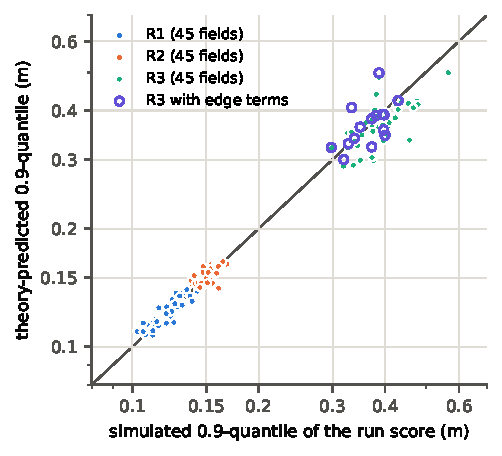
\includegraphics[width=\textwidth]{../../../figures/paper/fig_theory_vs_sim.pdf}
\caption{覆盖分数 0.9 分位数的预测值与仿真值（m，双对数坐标）。每点代表一块田，每种机型配置 45 块；两轴之间是模型与构建它所依据的仿真模型的比较。（a）解析模型（R3 含边界项）；（b）蒙特卡洛数字孪生（1000 次作业）。仿真值为 200 次独立作业的经验 0.9 分位数；阴影带为 ±10\%。}\label{fig:3}
\end{figure}

\textbf{有效性：B1～B4。} 此前 3 项预注册跨田块实验促成了比值形式的尺度（表 S30，附录 D.3～D.6）：B1 采用概率积分变换尺度，未通过；B2 的两项预期结论均成立，但主要得益于单次校准抽样下实际达到的无漏作业率；B3 部分成立。单次校准抽样下，R1 边际规则的无漏作业率为 0.844（B2）和 0.877（B3）。B4 将校准田块及其作业记录同时重抽 4000 次，全部 26 个单元（机型配置或混合机队 × 尺度 × 规则）均达标（边际平均值为 0.919～0.929，精确值为 0.923；表 S19a、图 S1）。因此，上述数值与单次抽样的波动相符。B4 无法检出可交换性不成立的情形。

\textbf{B5：混合机队（预注册）。} 4 项预注册预测全部成立。B5 将模型尺度与考虑机型配置的基线方法相比较，并分机型配置报告无漏作业率（表~\ref{tab:7}、图~\ref{fig:4}）。4 项预测为：（1）所有未拒绝给出裕量的尺度总体有效；（2）直接合并使 DGPS 配置的无漏作业率低于 0.85，而模型尺度使各机型配置均不低于 0.88；（3）校准田块为 25 块时，Mondrian 分组校准对超过 20\%（边际规则）和 95\%（PAC 规则）的田块拒绝给出裕量；（4）校准田块为 60 块时，模型尺度与考虑机型配置的基线方法相差在 0.5 pp 以内或更优，数字孪生与解析模型相差在 0.5 pp 以内。

\begin{table}[!htbp]
\centering
\footnotesize
\caption{实验 B5 结果（预注册）：135 块田组成的混合机队，重复抽样 4000 次；超额重叠率单位为 pp。所有未拒绝给出裕量的尺度总体均有效（边际平均值 0.896～0.925；PAC 规则下达标的重复抽样比例 0.892～0.955）。分机型配置的无漏作业率不在保证范围内；粗体表示低于 0.88（与表~\ref{tab:8} 规则相同）。Mondrian 的超额重叠率按给出裕量的田块计算。不含边界项的 XCE-T 为预注册尺度。完整结果见表 S26。}\label{tab:7}
\begin{tabularx}{\textwidth}{@{}>{\raggedright\arraybackslash\hsize=0.98\hsize}X>{\raggedright\arraybackslash\hsize=0.79\hsize}X>{\raggedright\arraybackslash\hsize=1.09\hsize}X>{\raggedright\arraybackslash\hsize=1.13\hsize}X@{}}
\toprule
\textbf{尺度} & \textbf{\(n=25\)：无漏作业率 R1 / R2 / R3（边际）} & \textbf{\(n=25\) 超额重叠率，边际 / PAC} & \textbf{\(n=60\) 超额重叠率，边际 / PAC} \\
\midrule
直接合并 & 0.999 / 0.998 / \textbf{0.779} & +29.19 / +63.97 & +17.12 / +37.98 \\
厂商规格 × 尺度律 & 0.944 / \textbf{0.840} / 0.993 & +12.95 / +23.09 & +9.93 / +14.98 \\
Mondrian（分机型配置） & 0.958 / 0.960 / 0.957 & 56\% / 100\% 的田块拒绝给出裕量 & +4.35 / 74\% 的田块拒绝给出裕量 \\
分机型配置尺度 & 0.939 / 0.958 / \textbf{0.842} & +4.57 / +19.94 & +1.29 / +6.42 \\
CQR（考虑机型配置） & 0.961 / 0.942 / \textbf{0.866} & +4.09 / +18.86 & +1.20 / +6.19 \\
\textbf{XCE-T}（解析模型） & 0.931 / 0.936 / 0.904 & \textbf{+2.89} / +14.56 & \textbf{+0.57} / +4.37 \\
\textbf{XCE-T}（含边界项） & 0.927 / 0.931 / 0.917 & +3.03 / \textbf{+13.69} & +0.63 / +4.36 \\
\textbf{XCE-MC}（蒙特卡洛数字孪生） & 0.924 / 0.929 / 0.913 & \textbf{+2.68} / \textbf{+13.76} & \textbf{+0.55} / \textbf{+4.19} \\
\bottomrule
\end{tabularx}
\end{table}

总体保证可能掩盖某一机型配置严重不足的情况：直接合并对 RTK 田块的无漏作业率达 0.999，对 DGPS 配置却仅为 0.779。边际规则下，在两种校准田块数下，模型尺度使各机型配置的实测无漏作业率均为 0.885～0.936（表 S26）。加入边界项后，在超额重叠率不变的情况下，DGPS 田块的边际平均无漏作业率或 PAC 达标比例由 0.834～0.904 提高到 0.899～0.924。Mondrian 分组校准每种机型配置至少需要 9 块（边际规则）或 22 块（PAC 规则）校准田块。3 种机型配置共用 25 块校准田块时，Mondrian 对 56\% 的目标田块（边际规则）和全部目标田块（PAC 规则）拒绝给出裕量。校准田块为 60 块时，边际规则下模型尺度的超额重叠率为 0.55～0.63 pp，考虑机型配置的学习尺度和经验尺度为 1.20～1.29 pp，Mondrian 为 4.35 pp。PAC 规则下三者依次为 4.2～4.4、6.2～6.4 和 12.2 pp，其中 Mondrian 只计其未拒绝的 26\% 田块。考虑机型配置的尺度使 DGPS 田块的无漏作业率仅为 0.82～0.87，原因是仅凭每块田 1 次作业学到的尺度，无法刻画 DGPS 更重的误差尾部。解析模型与数字孪生在各单元中相差均在 0.8 pp 以内。

\begin{figure}[!htbp]
\centering
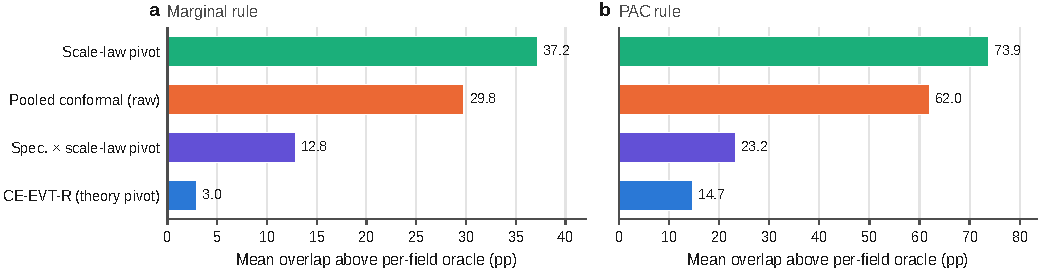
\includegraphics[width=\textwidth]{../../../figures/paper/fig_mixed_fleet.pdf}
\caption{实验 B5 结果。（a）（b）60 块校准田块时各尺度的平均超额重叠率（XCE-T 含边界项），分别对应边际规则和 PAC 规则（按给出裕量的田块计算；浅色柱表示对部分田块拒绝给出裕量的尺度）；（c）25 块校准田块、边际规则下 DGPS 田块的平均无漏作业率（虚线为 0.9）。}\label{fig:4}
\end{figure}

\subsection{鲁棒性}

\textbf{C1：模型失配（预注册）。} 设置 6 种仿真``真实场景''，改变实际作业条件，而所有归一化尺度仍采用标称模型：T1，间歇性局部湿软区，伴有重尾打滑脉冲；T2，牵引式农机具（挂接长度 5 m，下坡侧偏）；T3，车速 1.5～3.0 m/s，转向延迟 0.15 s，死区 0.3°；T4，GNSS 误差增大为 1.5 倍；T5，地形坡度降为原来的四分之一（平整格田）；T6，T1～T4 的组合。对每块田和每种变体，均按真实场景仿真 200 次校准作业，并计算 28 个裕量下的无漏作业率和重叠率（即裕量曲线）（表~\ref{tab:8}）。4 项预注册预测中，没有一项在全部变体下都成立（表 S27）。

\begin{table}[!htbp]
\centering
\footnotesize
\caption{实验 C1（预注册）。模型偏差为标称解析模型分位数（含边界项）与真实分位数之比的对数均值，每种机型配置 45 块田。混合机队：边际规则，60 块校准田，重复抽样 2000 次。CE-q：每块田 500 次重复抽样的均值。粗体：总体不大于 0.895，或某一机型配置低于 0.88。†为负值是因为 DGPS 田块裕量不足（无漏作业率 0.852～0.885），并非效率提高。}\label{tab:8}
\begin{tabularx}{\textwidth}{@{}l>{\raggedright\arraybackslash\hsize=0.81\hsize}X>{\raggedright\arraybackslash\hsize=0.85\hsize}X>{\raggedright\arraybackslash\hsize=1.54\hsize}X>{\raggedright\arraybackslash\hsize=0.81\hsize}X@{}}
\toprule
\textbf{真实场景} & \textbf{模型偏差 \(\log(\hat q/q)\)，R1 / R2 / R3} & \textbf{XCE-T 无漏作业率：总体 / DGPS（直接合并 DGPS）} & \textbf{超额重叠率/pp：XCE-T / XCE-MC / 规格 × 尺度 / Mondrian / 直接合并} & \textbf{CE-q（\(n=100\)）无漏作业率 R1 / R2 / R3} \\
\midrule
标称 & +0.01 / +0.00 / +0.01 & 0.902 / 0.899（\textbf{0.718}） & 0.63 / 0.55 / 9.93 / 4.35 / 17.12 & 0.896 / 0.909 / 0.898 \\
T1 局部湿软区 & −0.73 / −0.72 / −0.02 & \textbf{0.895} / 0.984（\textbf{0.823}） & 2.39 / 1.77 / 45.53 / 23.49 / 7.81 & \textbf{0.893 / 0.891} / 0.897 \\
T2 牵引式农机具 & +0.42 / +0.43 / +0.09 & 0.903 / \textbf{0.808}（\textbf{0.716}） & 0.49 / 0.52 / 3.93 / 3.81 / 17.86 & 0.900 / 0.903 / 0.902 \\
T3 车速、延迟 & +0.00 / +0.01 / −0.99 & 0.903 / \textbf{0.853}（\textbf{0.801}） & −18.07† / −17.51† / −9.02† / 40.68 / 3.93 & 0.899 / 0.899 / 0.924 \\
T4 GNSS × 1.5 & −0.04 / −0.02 / −0.35 & 0.901 / \textbf{0.803}（\textbf{0.711}） & 0.69 / 0.75 / 7.66 / 6.99 / 42.73 & 0.896 / 0.902 / 0.897 \\
T5 平整地形 & −0.01 / +0.01 / +0.02 & 0.902 / 0.908（\textbf{0.717}） & 0.56 / 0.47 / 9.99 / 3.98 / 16.47 & 0.904 / 0.899 / 0.904 \\
T6 组合 & −0.48 / −0.45 / −1.82 & 0.905 / \textbf{0.780}（\textbf{0.753}） & 14.09 / 12.33 / 8.71 / 51.01 / 58.34 & 0.908 / 0.899 / 0.949 \\
\bottomrule
\end{tabularx}
\end{table}

\emph{有效性。} 6 种变体中有 5 种，所有归一化尺度总体上仍然有效。T1 的打滑脉冲使 RTK 所需裕量约增加 1 倍。该变体下，校准田为 60 块时，各尺度的总体边际无漏作业率降至 0.892～0.895（判据为 0.895，精确期望值为 0.902）；100 次作业的 CE-q 为 0.893（R1）和 0.891（R2）。原因在推广环节而非共形校准环节：基准裕量依据标称训练田块设定，而多数田块上实施的 RTK 裕量超过了基准裕量。推广检查本会拒绝这些裕量，并在更宽的基准规划上重新校准；重新校准后的重叠率本文未作计算。

\emph{模型精度。} 仅对误差重新缩放的失配不影响模型的实用性。牵引式农机具条件下，模型对裕量的预测偏大约 50\%（对数偏差 +0.42；农机具对拖拉机的横向误差起低通滤波作用）；GNSS 精度下降时，模型对 DGPS 裕量的预测偏小（−0.35）；平整地形条件下，模型仍然准确。在这些变体中，XCE-T 仍是效率最高的尺度（超额重叠率 0.5～0.7 pp，其余尺度为 3.8～42.7 pp）。改变误差结构的失配则不然：存在局部湿软区时，实际 RTK 裕量为模型预测值的 2 倍；车速提高并存在转向延迟和死区时，DGPS 控制回路失稳，实际裕量为模型预测值的 2.7 倍；组合变体中，厂商规格尺度的效率反而更高（8.7 pp 对 14.1 pp）。蒙特卡洛数字孪生与解析模型基于相同假设，在上述情形下同样失效。

\emph{分机型配置的无漏作业率。} 当失配对某一机型配置的影响大于其他配置时（T2、T3、T4 和 T6），模型尺度不再能使各机型配置的无漏作业率趋于一致：DGPS 田块为 0.78～0.85，优于直接合并（0.71～0.80），但仍低于目标值。

\textbf{C2：地头绕行（预注册）。} 主体实验中，只有最外侧行程覆盖作业主区的边缘。C2 在每条边外增加一圈地头绕行，规划时使其与作业主区重叠 \(\lambda\)，并在田内行程完成后行驶。不设地头绕行时，由田块边界项决定覆盖分数的作业所占比例为 1.0\%（R1）、0.8\%（R2）和 10.0\%（R3）；设地头绕行后为 0.1\%、0.1\% 和 1.9\%。地头绕行不改变 RTK 下所需裕量，使 DGPS 下所需裕量降低约 6\%（理想裕量 0.391 → 0.366 m；重叠率 15.12\% → 14.01\%）。2 项预注册预测均成立：DGPS 下边界项所占比例低于预注册阈值 50\%（该阈值是在预期边界项将主导 DGPS 漏作业时设定的；即使不设地头绕行，实测比例也只有 10.0\%）；加入地头绕行后 CE-q 仍然有效（边际均值 0.897～0.902；PAC 规则达标率 0.885～0.907；表 S28）。

\subsection{校准零漏作业裕量的经济代价}

在``以 0.9 的概率不出现任何漏作业带''这一事件中，1 cm 的细缝与 1 m 宽的漏作业带同等计入。设 \(r\) 为单位面积漏作业损失与单位面积重复作业损失之比（对以节约农资为目的的作业，即漏作业带上损失的产量或防治效果价值与农资成本之比）。某一裕量的期望成本（以占作业主区面积的百分比计）为重叠率 \(+\ r\times\) 漏作业面积。该成本只计入农资成本：重叠带来的额外行程、时间和燃油，以及重复施用造成的危害（倒伏、除草剂药害），都会使重叠的代价更高，并提高零漏作业裕量开始合算的成本比；而漏作业细缝可能部分由相邻行作物补偿，漏除的杂草则可能连续多年结籽。表~\ref{tab:9} 和图~\ref{fig:5} 基于每种机型配置 45 块测试田的裕量曲线计算该成本（标称模型，描述性分析）。

\begin{table}[!htbp]
\centering
\scriptsize
\caption{期望成本（重叠率 \% + \(r\) × 漏作业面积 \%），描述性分析。``校准裕量（理想）''为各田块的理想裕量，即精确校准的方法所应实施的裕量；成本最优裕量为在给定测试分布下使各田块期望成本最小的裕量（仅作参照，并非一种方法）。由于田块集合不同（45 块对 30 块），厂商经验规则的重叠率与表~\ref{tab:6} 不同。完整结果见表 S29。}\label{tab:9}
\begin{adjustbox}{max width=\textwidth}
\begin{tabular}{@{}lllllllll@{}}
\toprule
\textbf{机型配置} & \textbf{策略} & \textbf{无漏作业率} & \textbf{重叠率/\%} & \textbf{漏作业面积/\%} & \textbf{成本，\(r=10\)} & \textbf{\(r=30\)} & \textbf{\(r=100\)} & \textbf{\(r=300\)} \\
\midrule
R1 & 厂商经验规则 & 0.000 & 2.12 & 0.160 & 3.72 & 6.92 & 18.10 & 50.04 \\
\textasciitilde{} & 农户经验裕量 & 0.882 & 9.05 & 0.001 & 9.06 & 9.07 & 9.11 & 9.24 \\
\textasciitilde{} & 校准裕量，\(\varepsilon=0.1\)（理想） & 0.900 & 8.91 & 0.001 & 8.92 & 8.93 & 8.98 & 9.11 \\
\textasciitilde{} & 成本最优裕量 & 0.02～0.50 & 2.5～6.0 & \textasciitilde{} & \textbf{3.54} & \textbf{4.69} & \textbf{5.92} & \textbf{7.10} \\
R2 & 厂商经验规则 & 0.000 & 5.38 & 0.336 & 8.74 & 15.45 & 38.95 & 106.09 \\
\textasciitilde{} & 农户经验裕量 & 0.844 & 23.02 & 0.001 & 23.03 & 23.05 & 23.11 & 23.30 \\
\textasciitilde{} & 校准裕量，\(\varepsilon=0.1\)（理想） & 0.900 & 24.93 & 0.001 & 24.94 & 24.95 & 24.99 & 25.11 \\
\textasciitilde{} & 成本最优裕量 & 0.00～0.32 & 5.9～15.0 & \textasciitilde{} & \textbf{8.58} & \textbf{11.58} & \textbf{14.78} & \textbf{17.75} \\
R3 & 厂商经验规则 & 0.437 & 7.56 & 0.112 & 8.68 & 10.91 & 18.73 & 41.07 \\
\textasciitilde{} & 农户经验裕量 & 0.853 & 13.35 & 0.033 & 13.68 & 14.33 & 16.62 & 23.16 \\
\textasciitilde{} & 校准裕量，\(\varepsilon=0.1\)（理想） & 0.900 & 15.10 & 0.026 & 15.36 & 15.88 & 17.69 & 22.87 \\
\textasciitilde{} & 成本最优裕量 & 0.21～0.89 & 4.6～14.4 & \textasciitilde{} & \textbf{7.15} & \textbf{10.31} & \textbf{15.21} & \textbf{21.90} \\
\bottomrule
\end{tabular}
\end{adjustbox}
\end{table}

\begin{figure}[!htbp]
\centering
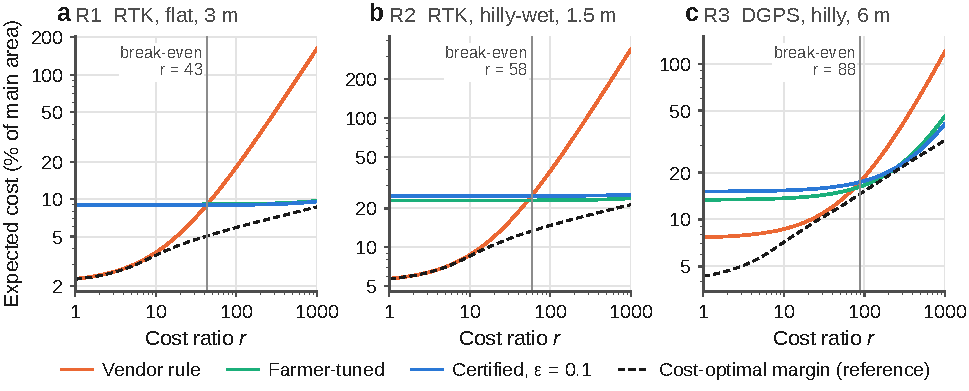
\includegraphics[width=\textwidth]{../../../figures/paper/fig_cost.pdf}
\caption{期望成本随成本比 \(r\) 的变化（双对数坐标）。对比策略为厂商经验规则、农户经验裕量、\(\varepsilon=0.1\) 时的校准裕量（理想裕量）和成本最优裕量；（a）～（c）分别为各机型配置测试田上的均值。竖线为盈亏平衡成本比 \(r_\mathrm{be}\)，成本比高于该值时，校准裕量比厂商经验规则更经济。}\label{fig:5}
\end{figure}

由此可得 3 点结论：

\begin{enumerate}
\def\labelenumi{\arabic{enumi}.}
\tightlist
\item
  与厂商经验规则相比，校准的零漏作业裕量仅在成本比超过盈亏平衡点 \(r_\mathrm{be}\approx43\)（R1）、58（R2）和 88（R3）时才更经济；若改用实验 A1 中各机型配置的结果，盈亏平衡点为 31～35（RTK）和 88～117（DGPS）。
\item
  RTK 下，成本最优裕量容许频繁但极细微的漏作业（细缝占面积的 0.004\%～0.03\%）：即使 \(r=300\)，其无漏作业率也仅为 0.50（R1）和 0.32（R2）。只有在漏作业带较宽的 DGPS 下，其无漏作业率才接近 0.9（\(r=300\) 时为 0.89）。
\item
  农机具作业幅宽较窄时，漏缝容许宽度更有效：将要求改为``无宽于 2 cm 的漏缝''，裕量可减小 1 cm，R1～R3 的重叠率分别降低 0.9、2.0 和 0.4 pp；容许宽度取 5 cm 时，分别降低 2.0、5.0 和 1.1 pp。
\end{enumerate}

本文未估计 \(r\) 的取值。仅作假设性举例：若某一施肥带漏施会损失三分之一的作物，而该作物价值为肥料成本的 5 倍，则 \(r\approx1.7\)；若漏作业会引发监管、检疫或抗性治理方面的成本，\(r\) 可达数百。低于盈亏平衡点时，只要事先确定 \(\varepsilon\) 或 \(\tau\)（第 3.7 节），校准仍可给出更经济裕量所对应的漏作业概率。以期望漏作业面积为对象的共形风险控制 \citep{angelopoulos2024crc} 可直接以成本为目标，但其有限样本项 \(B/(n+1)\)（\(B\) 为最大可能损失）会超过所关心的漏作业面积水平（0.01\%～0.1\%），除非有数千次作业可用。

\section{讨论}

\subsection{实验对可靠性保证的检验}

实施裕量低于基准裕量且各行程独立导航时，实测无漏作业率与目标一致（带推广检查的 A1；A2、B4、B5 和 C2 中边际均值为 0.896～0.943）。无漏作业率低于目标的情形有两种：一是实施裕量超过基准裕量（C1 局部湿软区变体中为 0.891～0.895），推广检查可防止这种情况；二是跟随上一行程的导航方式使行程相互耦合（0.850），本方法中没有任何检查能发现这种情况。模型尺度不影响对田块平均的保证，但决定了效率、推广检查拒绝给出裕量的频率，以及无漏作业率在各机型配置间的分布（直接合并时 DGPS 为 0.78；标称仿真模型下采用模型尺度时，各机型配置为 0.885～0.936）。

\subsection{方法的优势与不足}

\emph{有目标田块数据时}，CE+ 达到目标所需的重叠率比 2 种共形规划方法低 4\%～55\%，后者偏于保守。与调校良好的生产实践相比，增益很小：农户经验裕量在 R1 中比 CE+ 多 0.8 pp 重叠率，在 R2 和 R3 中少 2.2～2.6 pp，但无漏作业率较低（20\%～70\% 的田块达到目标）；此时本方法的价值在于给出明确的漏作业概率。\emph{无目标田块数据时}，在所比较的尺度中，只有模型尺度既使各机型配置都接近目标，又保持高效（比理想裕量高 0.6 pp，考虑机型配置的基线方法高 1.2～4.4 pp，直接合并高 17 pp）；数字孪生与解析模型效果相当，且已有仿真模型时更易构建。不过，在同一机型配置内，相同无漏作业率下各种田块级尺度之间仅相差 0.1～0.4 pp（事后分析；附录 D.4），这与理想尺度下的裕量膨胀一致（第 3.8 节）。作业次数少时，PAC 规则代价较高（\(n=22\) 时为 3～19 pp）。\(\varepsilon=0.1\) 的零漏作业裕量在成本比超过约 40～90 时虽比厂商经验规则更经济，但只有当单位漏作业损失达到单位重复作业损失的数百倍时才是成本最优选择（R3：\(r=300\) 时无漏作业率为 0.888；R1：0.495）；对大多数以节约农资为目的的作业，采用漏缝容许宽度或更大的 \(\varepsilon\) 更好。

\subsection{与生产实践的关系}

校准所得裕量大于田间经验：R1 的理想裕量约为 12 cm，约为厂商经验规则裕量（2.5 cm）的 5 倍；R2 约 25\% 的重叠率，则源于在 1.5 m 农机具上采用相近的绝对裕量（约 15 cm）。原因有三。第一，本文的事件是整块田一次作业无任何漏作业，要求数十至数百个相邻行程对全部保持覆盖，而不是 95\% 的行间精度。第二，RTK 序列中有 16\% 的浮点解历元和持续数分钟的错误固定解（表~\ref{tab:3}），带完整性监测的导航终端可能会对其发出警示，因此仿真的误差尾部可能比商用 RTK 偏重。第三，30 m 地形模型使平整的水田格田带有坡度。另一方面，厂商经验规则的漏作业仅占作业主区面积的 0.12\%～0.64\%；其宽度未作记录，较窄的漏缝可能部分由喷雾飘移或撒布幅弥补。所有比较均假设无人修补可见的漏缝，因此适用于无人驾驶或无人监管的作业。自动分段控制降低了重叠的代价，因而会提高 \(r\)。本方法的输出是单个导航参数，即行距 \(w-2\hat\lambda\)，可直接纳入现有导航终端和任务控制器的工作流程；实际应用的主要要求是作业记录需有独立的农机具位置参考，例如安装在农机具上的 PPK 流动站。

\subsection{局限性}

\begin{enumerate}
\def\labelenumi{\arabic{enumi}.}
\tightlist
\item
  \textbf{仅为仿真研究。} 田块边界、地形和 GNSS 误差均来自真实数据，作业过程则为仿真：车辆采用运动学模型，主要实验中农机具为刚性连接，行驶速度单一，中国田块上施加的是美国 CORS 站的误差，地形坡度取自 30 m 地形模型。模型设定有误时（C1），可靠性保证基本仍成立，而模型的效率优势只在失配仅对误差重新缩放时得以保持。田间验证不在本文范围内。
\item
  \textbf{真值。} 计算覆盖分数需要农机具的真实位置；参考基准的误差会进入覆盖分数。
\item
  \textbf{耦合假设。} CE-q、CE+ 和 XCE 依赖该假设；跟随上一行程的导航方式不满足该假设。
\item
  \textbf{可交换性。} 校准田块与目标田块必须来自同一总体；同一天作业的田块具有相同的 GNSS 条件，本文实验未对此建模。
\item
  \textbf{适用范围。} 仅限作业主区内的直线平行行程，不涉及曲线导航线、障碍物和地头本身；零漏作业事件不考虑漏作业的大小。
\end{enumerate}

\subsection{应用建议}

\begin{enumerate}
\def\labelenumi{\arabic{enumi}.}
\tightlist
\item
  在查看任何覆盖分数之前，先确定成本比 \(r\)，再确定 \(\varepsilon\) 和 \(\tau\)。成本比低于约 40～90（按 A1 结果为 31～117）时，\(\varepsilon=0.1\) 的零漏作业裕量比厂商经验规则成本更高，应采用漏缝容许宽度或更大的 \(\varepsilon\)。
\item
  记录作业时应同时获取农机具位置的独立真值，并只合并可比的作业（表~\ref{tab:1}）。
\item
  基准规划的行程数应不少于实施规划，切勿采用零裕量规划。
\item
  每块田有不少于 22 次作业记录（边际规则下为 9 次，代价是 1～8 pp 的额外重叠率）时，直接在该田块上校准；记录更少时，以模型尺度跨田块校准（采用蒙特卡洛数字孪生即可），逐机型配置检验无漏作业率，并用每种机型配置的少量作业记录验证模型。
\item
  执行推广检查；若 \(\hat\lambda>\lambda_\mathrm{ref}\)，在更宽的基准规划上重新校准。
\item
  在导航终端中输入行距 \(w-2\hat\lambda\)；更换主机、农机具、接收机、差分改正源或作业速度后重新校准。与作业主区重叠的地头绕行可消除大部分由田块边界主导的漏作业。
\end{enumerate}

\section{结论}

本文提出共形收缩法，由作业记录校准农田全覆盖规划的行间重叠量。该方法按选定的``一次作业出现任何漏作业带''的概率设定裕量；反之，对任意选定的裕量或漏缝容许宽度，也能给出其漏作业概率。每次作业归结为一个覆盖分数，即包括田块边界在内的实际行程覆盖半径；无作业历史的田块以车辆---地形---GNSS 模型为统一尺度跨田块校准。只要各次作业（或各田块）可交换，所得上界不需要对误差分布作假设。基于真实田块边界、地形和 GNSS 误差的预注册仿真实验表明：

（1）每块田有 100 次作业记录时，本方法达到目标漏作业水平，且在相同标称水平下，重叠率比 2 种共形规划方法低 4\%～55\%（采用推广检查时为 4\%～59\%）。

（2）无目标田块数据时，在标称仿真模型下，模型尺度（解析模型或蒙特卡洛数字孪生）使混合机队中各机型配置的实测无漏作业率为 0.885～0.936，重叠率比逐田块理想裕量高 0.6 pp，而考虑机型配置的基线方法高 1.2～4.4 pp。

（3）这一效率优势在牵引式农机具、GNSS 精度下降和平整地形条件下依然存在，在重尾打滑和转向失稳条件下则消失。未达到目标漏作业水平的情形有两种：实施裕量超过基准裕量，推广检查可排除这种情况；跟随上一行程的导航方式不满足耦合假设。

（4）仅当单位面积漏作业损失约超过重复作业损失的 40～90 倍时，零漏作业裕量才比厂商经验规则更经济；否则，采用漏缝容许宽度或放宽漏作业水平更为合适，且同一校准结果可给出所选设置的漏作业概率。

下一步将以独立真值开展田间验证。



\section*{数据可用性}
代码、处理后的输入数据、预注册文件（含版本控制时间戳）、原始结果以及生成全部表格和图的脚本均存放于项目代码仓库，仓库 README 提供了复现指南；归档版本将在论文录用后获得 DOI。输入数据均为公开数据，包括田---路轨迹数据集 \citep{wu2023}、Copernicus GLO-30 \citep{esa2021}、NOAA CORS 观测数据 \citep{noaacors} 以及 \citet{tang2022} 的车辆 GNSS/INS 数据。

\section*{作者贡献声明（CRediT）}
［待作者填写。］

\section*{利益冲突声明}
作者声明不存在可能影响本文工作的已知经济利益冲突或个人关系。

\section*{写作过程中使用生成式人工智能及相关技术的声明}
［待作者按期刊要求填写。］

\section*{致谢}
［资助来源。］

\section*{补充材料}
证明、理论细节、实验细节与完整表格见补充材料（英文）。

\bibliographystyle{elsarticle-harv}
\bibliography{refs}
\end{document}
